\documentclass[margin=5mm]{standalone}
\usepackage[dvipsnames]{xcolor}
\usepackage{pgfplots}
\usepackage{tikz}

\pgfplotsset{compat=1.18}
\begin{document}

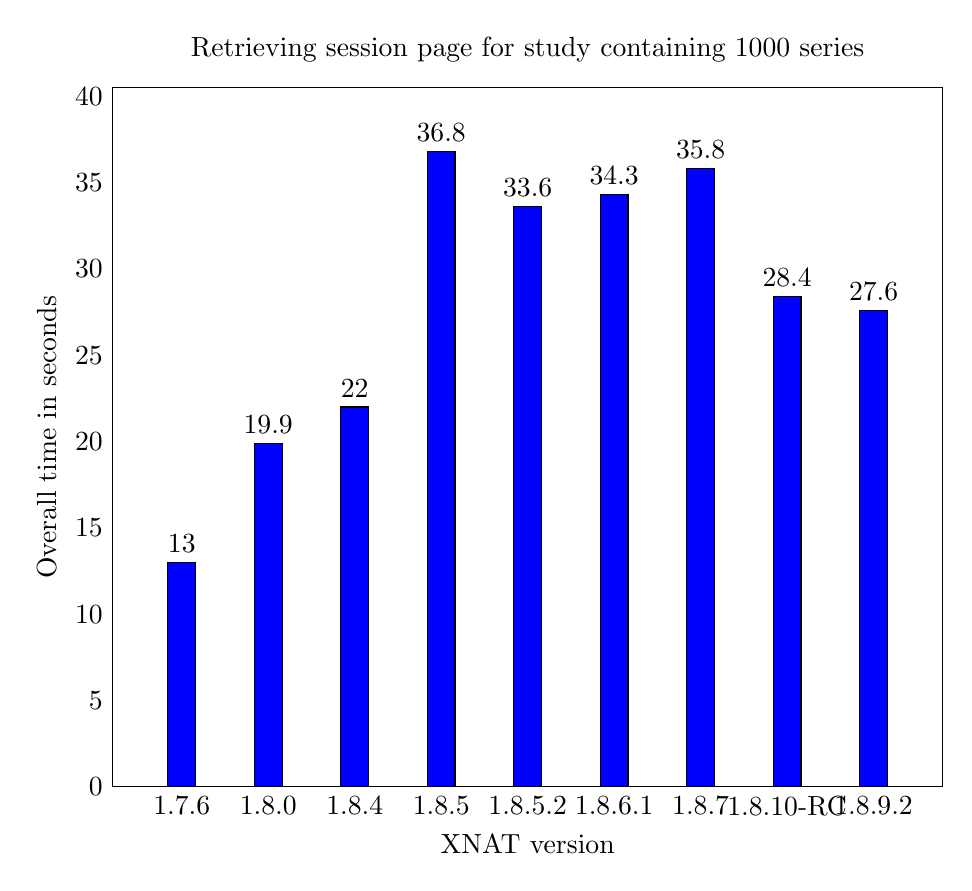
\begin{tikzpicture}
    \begin{axis}[
        width = \textwidth,
        xlabel = XNAT version,
        ylabel = Overall time in seconds,
        symbolic x coords = {1.7.6,1.8.0,1.8.4,1.8.5,1.8.5.2,1.8.6.1,1.8.7,1.8.10-RC,1.8.9.2},
        nodes near coords,
        xtick = {1.7.6,1.8.0,1.8.4,1.8.5,1.8.5.2,1.8.6.1,1.8.7,1.8.10-RC,1.8.9.2},
        ymin = 0,
        xtick pos = left,
        ytick pos = left,
        xticklabel style = {major tick length = 0pt},
        title = {Retrieving session page for study containing 1000 series}]
        \addplot[ybar,fill=blue] coordinates {(1.7.6, 13.0)};
        \addplot[ybar,fill=blue] coordinates {(1.8.0, 19.9)};
        \addplot[ybar,fill=blue] coordinates {(1.8.4, 22.0)};
        \addplot[ybar,fill=blue] coordinates {(1.8.5, 36.8)};
        \addplot[ybar,fill=blue] coordinates {(1.8.5.2, 33.6)};
        \addplot[ybar,fill=blue] coordinates {(1.8.6.1, 34.3)};
        \addplot[ybar,fill=blue] coordinates {(1.8.7, 35.8)};
        \addplot[ybar,fill=blue] coordinates {(1.8.10-RC, 28.4)};
        \addplot[ybar,fill=blue] coordinates {(1.8.9.2, 27.6)};
    \end{axis}
\end{tikzpicture}

\end{document}